\documentclass[11pt]{article}
\usepackage{graphicx}
\usepackage{hyperref}
\usepackage{appendix}
\usepackage{amsmath}
\usepackage{amsthm}
\usepackage[version=3]{mhchem}
\usepackage{amssymb}
\usepackage{float}
\usepackage{multirow}
\usepackage{commath}
\usepackage{booktabs}
\renewcommand{\arraystretch}{1.2}
\usepackage{siunitx}
\sisetup{detect-all}
\usepackage{listings}
\usepackage{color} %red, green, blue, yellow, cyan, magenta, black, white
\definecolor{mygreen}{RGB}{28,172,0} % color values Red, Green, Blue
\definecolor{mylilas}{RGB}{170,55,241}
\usepackage[a4paper,margin=20mm]{geometry}
\numberwithin{equation}{section}
\setlength{\parskip}{\baselineskip}
\setlength{\parindent}{0pt}
\hypersetup{
    colorlinks=true,
    linkcolor=black,
    filecolor=black,      
    urlcolor=black,
    citecolor=black
}
\urlstyle{same}
\begin{document}
\title{\textbf{UCL Mechanical Engineering 2020/2021}\\MECH0011 Final Coursework}
\author{NCWT3}
\maketitle
\begin{table}[H]
    \centering
    \begin{tabular}{@{}llllll@{}}
        \toprule
        Boat speed & Hydrofoil & Angle of & Hydrofoil & Average & $x_c/R$, $y_c/R$,\\
        $V_w$ (m/s) & wingspan $b$ (m) & attack (deg) & selected & chord $\bar{c}$ (m) & $R$\\
        \midrule
        11 & 2 & 0 & RG 8 Airfoil & & \\
        \bottomrule
        \end{tabular}
\end{table}
\tableofcontents
\listoffigures
\section{Question 1}
\subsection{a}
The data was imported into MATLAB and the shape of the hydrofoil, the chord line and the mean camber line were plotted for all four hydrofoils.
\lstset{language=Matlab,%
    %basicstyle=\color{red},
    breaklines=true,%
    morekeywords={matlab2tikz},
    keywordstyle=\color{blue},%
    morekeywords=[2]{1}, keywordstyle=[2]{\color{black}},
    identifierstyle=\color{black},%
    stringstyle=\color{mylilas},
    commentstyle=\color{mygreen},%
    showstringspaces=false,%without this there will be a symbol in the places where there is a space
    numbers=left,%
    numberstyle={\tiny \color{black}},% size of the numbers
    numbersep=9pt, % this defines how far the numbers are from the text
    emph=[1]{for,end,break},emphstyle=[1]\color{red}, %some words to emphasise
    %emph=[2]{word1,word2}, emphstyle=[2]{style},    
}
\lstinputlisting{./mCode/q1a.m}
\begin{figure}[H]
    \centering
    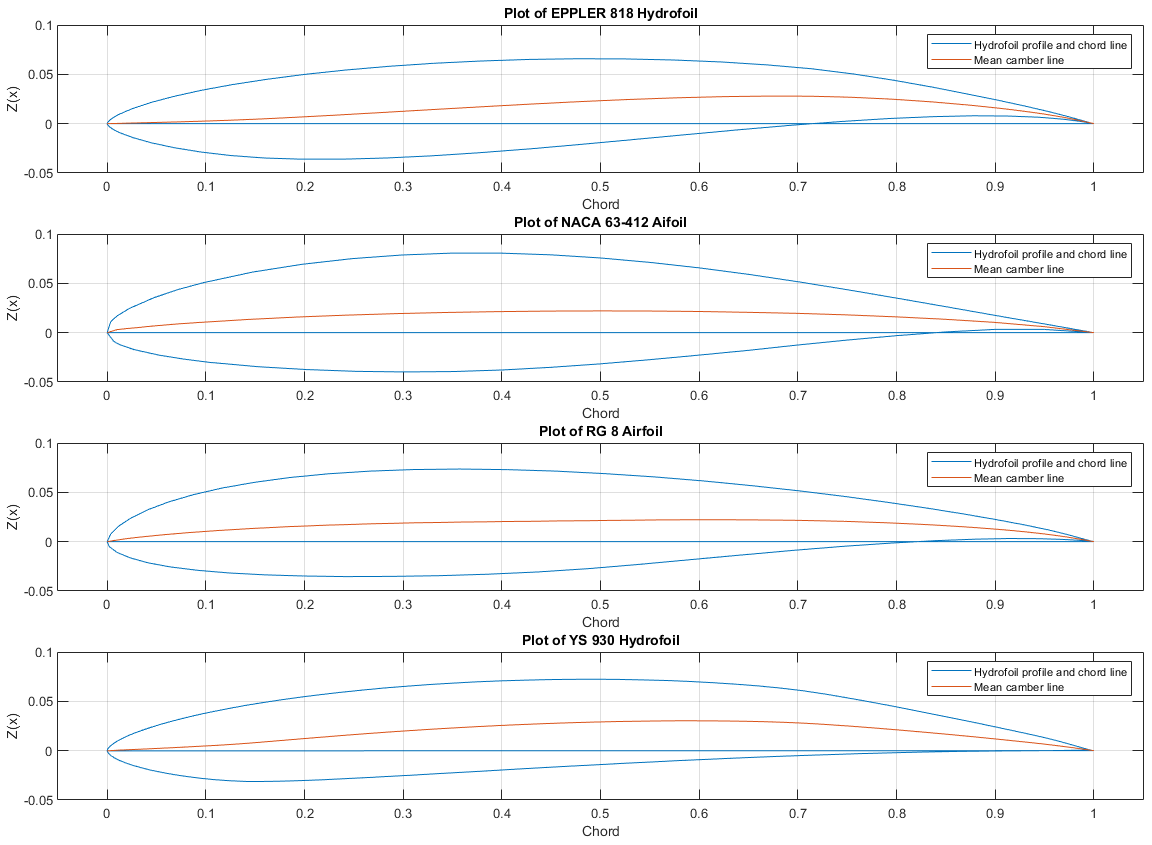
\includegraphics[width = \textwidth]{./img/q1a.png}
    \caption{Graphs to show hydrofoil shape, chord line and mean camber line for four different hydrofoils.}
    \label{fig:q1a}
\end{figure}
\subsection{b}
MATLAB was used to calculate the lift-to-drag ratio for each hydrofoil.
\lstset{language=Matlab,%
    %basicstyle=\color{red},
    breaklines=true,%
    morekeywords={matlab2tikz},
    keywordstyle=\color{blue},%
    morekeywords=[2]{1}, keywordstyle=[2]{\color{black}},
    identifierstyle=\color{black},%
    stringstyle=\color{mylilas},
    commentstyle=\color{mygreen},%
    showstringspaces=false,%without this there will be a symbol in the places where there is a space
    numbers=left,%
    numberstyle={\tiny \color{black}},% size of the numbers
    numbersep=9pt, % this defines how far the numbers are from the text
    emph=[1]{for,end,break},emphstyle=[1]\color{red}, %some words to emphasise
    %emph=[2]{word1,word2}, emphstyle=[2]{style},    
}
\lstinputlisting{./mCode/q1b.m}
\begin{figure}[H]
    \centering
    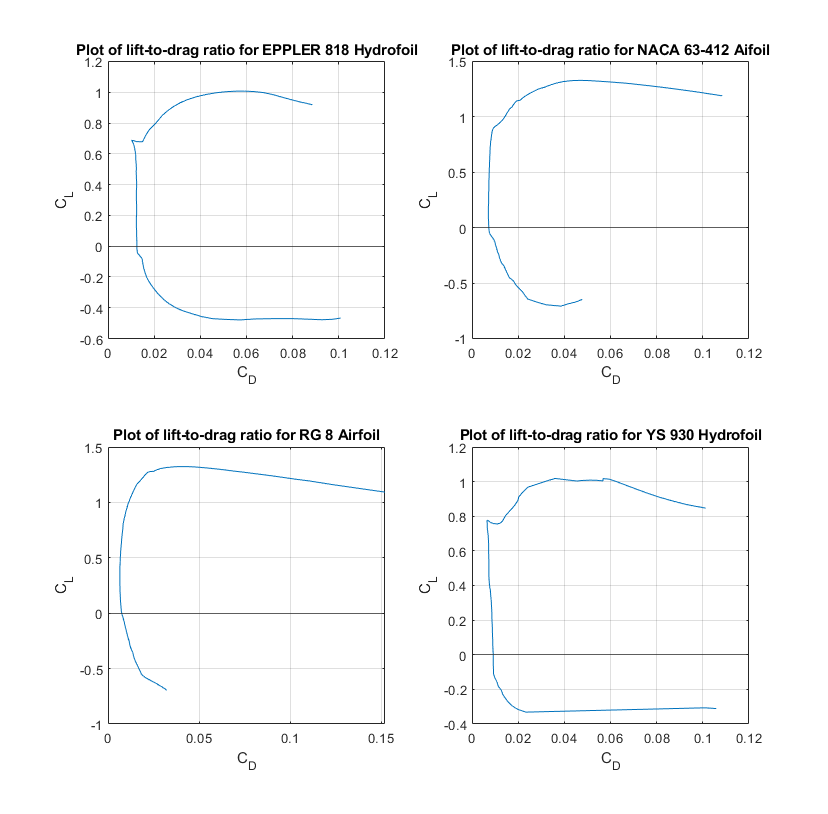
\includegraphics[height = 10cm]{./img/q1b.png}
    \caption{Graph to show lift-to-drag ratio for four different hydrofoils.}
    \label{fig:q1b}
\end{figure}
\subsection{c}
At a low angle of attack, the flow is attached to the hydrofoil and separates close to the trailing edge, leaving a small wake. The streamlined shape of the hydrofoil exerts a large shear force on the flow passing over it, leading to a large skin drag but low form drag. As we increase the angle of attack, the flow separation moves along the top of the hydrofoil. This decreases the shear force acting on the hydrofoil and the skin drag starts to reduce, with form drag increasing. At the stall angle, the pressure distribution along the top of the hydrofoil dramatically changes due to flow separation, suction pressure is mostly/all lost and a large wake with turbulent effects is present. The primary drag effect here is now form drag, as the flow is not attached along the length of the hydrofoil surface.
\subsection{d}
MATLAB was used to calculate each of the variables for each hydrofoil.
\lstset{language=Matlab,%
    %basicstyle=\color{red},
    breaklines=true,%
    morekeywords={matlab2tikz},
    keywordstyle=\color{blue},%
    morekeywords=[2]{1}, keywordstyle=[2]{\color{black}},
    identifierstyle=\color{black},%
    stringstyle=\color{mylilas},
    commentstyle=\color{mygreen},%
    showstringspaces=false,%without this there will be a symbol in the places where there is a space
    numbers=left,%
    numberstyle={\tiny \color{black}},% size of the numbers
    numbersep=9pt, % this defines how far the numbers are from the text
    emph=[1]{for,end,break},emphstyle=[1]\color{red}, %some words to emphasise
    %emph=[2]{word1,word2}, emphstyle=[2]{style},    
}
\lstinputlisting{./mCode/q1d.m}
\begin{table}[H]
    \centering
    \begin{tabular}{@{}llll@{}}
    \toprule
        & \multicolumn{3}{c}{Maximum}\\
        \cline{2-4}
        Hydrofoil& \% camber & \% thickness & lift coefficient \\
    \midrule
        EPPLER 818 Hydrofoil & 2.792 & 9.362  & 1.008 \\
        NACA 63-412 Aifoil   & 2.204 & 11.992 & 1.330 \\
        RG 8 Airfoil         & 2.226 & 10.795 & 1.323 \\
        YS 930 Hydrofoil     & 3.028 & 9.088  & 1.018 \\ 
    \bottomrule
    \end{tabular}
    \caption{Table to show maximum percentage camber and thickness and the maximum lift coefficient for four hydrofoils.}
\end{table}
\begin{table}[H]
    \centering
    \begin{tabular}{@{}llll@{}}
    \toprule
        & & Lift coefficient & Angle of attack $\alpha_0$\\
        Hydrofoil & Stall angle  & for $\alpha = \SI{0}{\degree}$ & corresponding to $C_L = 0$\\
    \midrule
        EPPLER 818 Hydrofoil & \SI{7.75}{\degree}  & 0.361 & \SI{-3}{\degree}    \\
        NACA 63-412 Aifoil   & \SI{13}{\degree}    & 0.338 & \SI{-3}{\degree}  \\
        RG 8 Airfoil         & \SI{12.75}{\degree} & 0.382 & \SI{-3}{\degree} \\
        YS 930 Hydrofoil     & \SI{9}{\degree}  & 0.391 & \SI{-3.75}{\degree}  \\ 
    \bottomrule
    \end{tabular}
    \caption{Table to show the stall angle, lift coefficient for $\alpha = \SI{0}{\degree}$ and the angle of attack $\alpha_0$ corresponding to $C_L = 0$ for four hydrofoils.}
\end{table}
The hydrofoils both have a higher percentage camber than the airfoils. They also have a lower percentage thickness than the airfoils. We can see that this leads to a reduction in the stall angle and subsequently their maximum lift coefficients are lower. However, we can see that they perform better at $\alpha = \SI{0}{\degree}$. This can be attributed to the fact that at small $\alpha$, larger camber generates more lift, at the expense of a smaller stall angle, as the boundary layer is more prone to separation at higher $\alpha$. However, increasing either percentage camber or thickness will increase $C_D$.
\subsection{e}
The RG 8 Airfoil was selected as it has a high stall angle, with a subsequently large maximum lift coefficient, the lift coefficient at $\alpha = \SI{0}{\degree}$ is also the second highest. We can calculate the lift on the hydrofoil using \ref{eq:q1e1}:
\begin{equation}
    L = \frac{1}{2}\rho C_L V_{w}^2 A \label{eq:q1e1}
\end{equation}
where $\rho$ is the density of seawater, $C_L$ is the lift coefficient for a given angle of attack, $V_w$ is the velocity of the fluid relative to the wing and $A$ is the projected surface area of the wing. The surface area $A$ can be found by integration:
\begin{align}
    A &= \int_{x_0}^{b + x_0} \left(-0.07x + c_0\right)\dif x\\
    A &= \left[-0.035x^2 + c_0x\right]_{x_o}^{b+x_0}
\end{align}
$x_0 = 0.1$ as given in the material. I have also selected $b = \SI{2}{\meter}$, hence:
\begin{align}
    A &= -0.035(2.1)^2 + c_0(2.1) + 0.035(0.1)^2 - c_0(0.1)\\
    A &= 2c_0 - 0.154 \label{eq:q1e2}
\end{align}
Substituting \ref{eq:q1e2} into \ref{eq:q1e1}:
\begin{align}
    L = \frac{1}{2}\rho C_L V_{w}^2 \left(2c_0 - 0.154\right)
\end{align}
Rearranging for $c_0$:
\begin{align}
    \left(2c_0 - 0.154\right) &= \dfrac{L}{\frac{1}{2}\rho C_L V_{w}^2}\\
    c_0 &= \dfrac{L}{\rho C_L V_{w}^2} + 0.077
\end{align}
The following values were used: $\rho = \SI{1036}{\kg\per\meter\cubed}$ \cite{b1}, $V_w = \SI{11}{\meter\per\second}$ (\SI{39.6}{\kilo\meter\per\hour}), $L = 2000\times 9.81 \approx \SI{20000}{\newton}$. MATLAB was used to plot the chord length against the angle of attack. As $V_w$ represents the upper speed limit of the boat, we want to select a low angle of attack, to reduce the amount of drag on the foil. Hence, the value for $C_L$ at $\alpha = 0$ will be used. 
\lstset{language=Matlab,%
    %basicstyle=\color{red},
    breaklines=true,%
    morekeywords={matlab2tikz},
    keywordstyle=\color{blue},%
    morekeywords=[2]{1}, keywordstyle=[2]{\color{black}},
    identifierstyle=\color{black},%
    stringstyle=\color{mylilas},
    commentstyle=\color{mygreen},%
    showstringspaces=false,%without this there will be a symbol in the places where there is a space
    numbers=left,%
    numberstyle={\tiny \color{black}},% size of the numbers
    numbersep=9pt, % this defines how far the numbers are from the text
    emph=[1]{for,end,break},emphstyle=[1]\color{red}, %some words to emphasise
    %emph=[2]{word1,word2}, emphstyle=[2]{style},    
}
\lstinputlisting{./mCode/q1e.m}
Our chord length is calculated to be $c_0 = \SI{0.4948}{\meter}$. We must now check whether this chord length is sufficient to lift the boat at lower speeds. In order to do this we require a high angle of attack, to generate more lift. The value for $C_L$ at \SI{11}{\degree} was used to test the lift at $\SI{6}{\meter\per\second}$ ($\SI{21.6}{\kilo\meter\per\hour}$) and MATLAB gives a lift value of \SI{20215}{\newton}, allowing the boat to be out of the water at lower speeds as well.
\section{Question 2}
\subsection{a}
\begin{figure}[H]
    \centering
    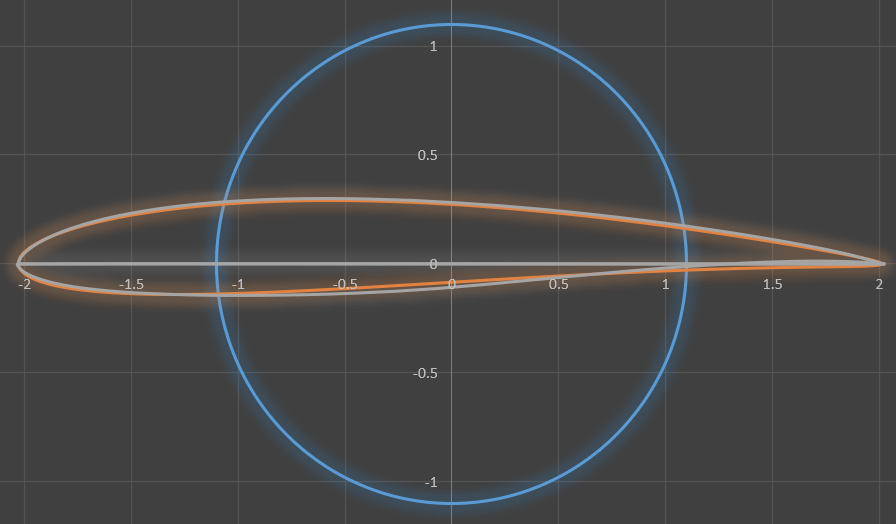
\includegraphics[height = 8cm]{./img/q2a.png}
    \caption{Graph to show conformal map onto RG 8 airfoil.}
    \label{fig:q2a}
\end{figure}
The Excel sheet from the Fluids lab was used to find values for $R$, $x_c$ and $y_c$. They were found to be:
\begin{align}
    R = 1.1, \; x_c = -0.065, \; y_c = 0.051     
\end{align}
\subsection{b}
\subsection{c}
\section{Question 3}
\subsection{a}
MATLAB was used to plot the boundary layer velocity profile.
\lstset{language=Matlab,%
    %basicstyle=\color{red},
    breaklines=true,%
    morekeywords={matlab2tikz},
    keywordstyle=\color{blue},%
    morekeywords=[2]{1}, keywordstyle=[2]{\color{black}},
    identifierstyle=\color{black},%
    stringstyle=\color{mylilas},
    commentstyle=\color{mygreen},%
    showstringspaces=false,%without this there will be a symbol in the places where there is a space
    numbers=left,%
    numberstyle={\tiny \color{black}},% size of the numbers
    numbersep=9pt, % this defines how far the numbers are from the text
    emph=[1]{for,end,break},emphstyle=[1]\color{red}, %some words to emphasise
    %emph=[2]{word1,word2}, emphstyle=[2]{style},    
}
\lstinputlisting{./mCode/q3a.m}
\begin{figure}[H]
    \centering
    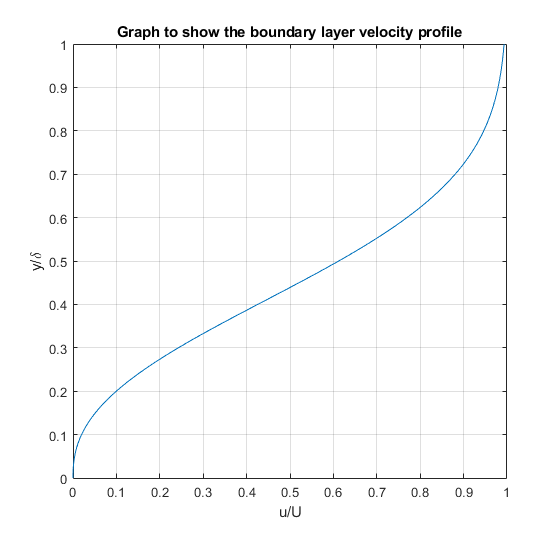
\includegraphics[height = 8cm]{./img/q3a.png}
    \caption{Graph to show boundary layer velocity profile.}
    \label{fig:q3a}
\end{figure}
\subsubsection{i}
One can expect to see this boundary layer velocity profile in the area  near the streamline separation point on the airfoil surface. We cannot see any negative velocity (indicative of backflow) nor do we see the viscous effects confined to a thing layer. For $\alpha = 0$, this would occur at the trailing edge of the airfoil. 
\subsubsection{ii}
Under stall conditions, our angle of attack is high and the airflow around the airfoil is prone to boundary layer separation early. Hence, we can expect to see this velocity profile close to the leading edge of the airfoil. The flow along the rest of the airflow is highly chaotic, hence we would only see this velocity profile near to the boundary layer separation point.
\subsection{b}
We can use the following formula to calculate the shape factor:
\begin{align}
    H = \dfrac{\int_0^{\delta}\left(1 - \dfrac{u}{U}\right)\dif y}{\int_0^{\delta}\left(\dfrac{u}{U}\left(1 - \dfrac{u}{U}\right)\right)\dif y}
\end{align}
Replacing our integrals with the trapezium method of integration:
\begin{align}
    H = \dfrac{\sum_{i=1}^{100}\left[\dfrac{\left(1-\dfrac{u}{U}\right)_i + \left(1-\dfrac{u}{U}\right)_{i+1}}{2}\cdot \left(\dfrac{y_{i+1}}{\delta} - \dfrac{y_i}{\delta}\right)\right]}{\sum_{i=1}^{100}\left[\dfrac{\left(\dfrac{u}{U}\left(1-\dfrac{u}{U}\right)\right)_i + \left(\dfrac{u}{U}\left(1-\dfrac{u}{U}\right)\right)_{i+1}}{2}\cdot \left(\dfrac{y_{i+1}}{\delta} - \dfrac{y_i}{\delta}\right)\right]}
\end{align}
This was implemented in MATLAB:
\lstset{language=Matlab,%
    %basicstyle=\color{red},
    breaklines=true,%
    morekeywords={matlab2tikz},
    keywordstyle=\color{blue},%
    morekeywords=[2]{1}, keywordstyle=[2]{\color{black}},
    identifierstyle=\color{black},%
    stringstyle=\color{mylilas},
    commentstyle=\color{mygreen},%
    showstringspaces=false,%without this there will be a symbol in the places where there is a space
    numbers=left,%
    numberstyle={\tiny \color{black}},% size of the numbers
    numbersep=9pt, % this defines how far the numbers are from the text
    emph=[1]{for,end,break},emphstyle=[1]\color{red}, %some words to emphasise
    %emph=[2]{word1,word2}, emphstyle=[2]{style},    
}
\lstinputlisting{./mCode/q3b.m}
The code yielded a shape factor $H = 4$. The shape factor of a BLVP upstream from the one in the supplementary material would be lower than the one given. This is because there will be a velocity at the boundary and shear stresses will be present, increasing momentum thickness. We would also see a reduction in the size of the thickness of the boundary layer, further reducing the shape factor. For a downstream BVLP, we would see a large separation of the flow from the boundary layer, hence a large displacement thickness. As there is no longer a flow of fluid at the boundary of the airfoil, there will be a large deficit of momentum; combined these factors would increase the shape factor. 
\begin{figure}[H]
    \centering
    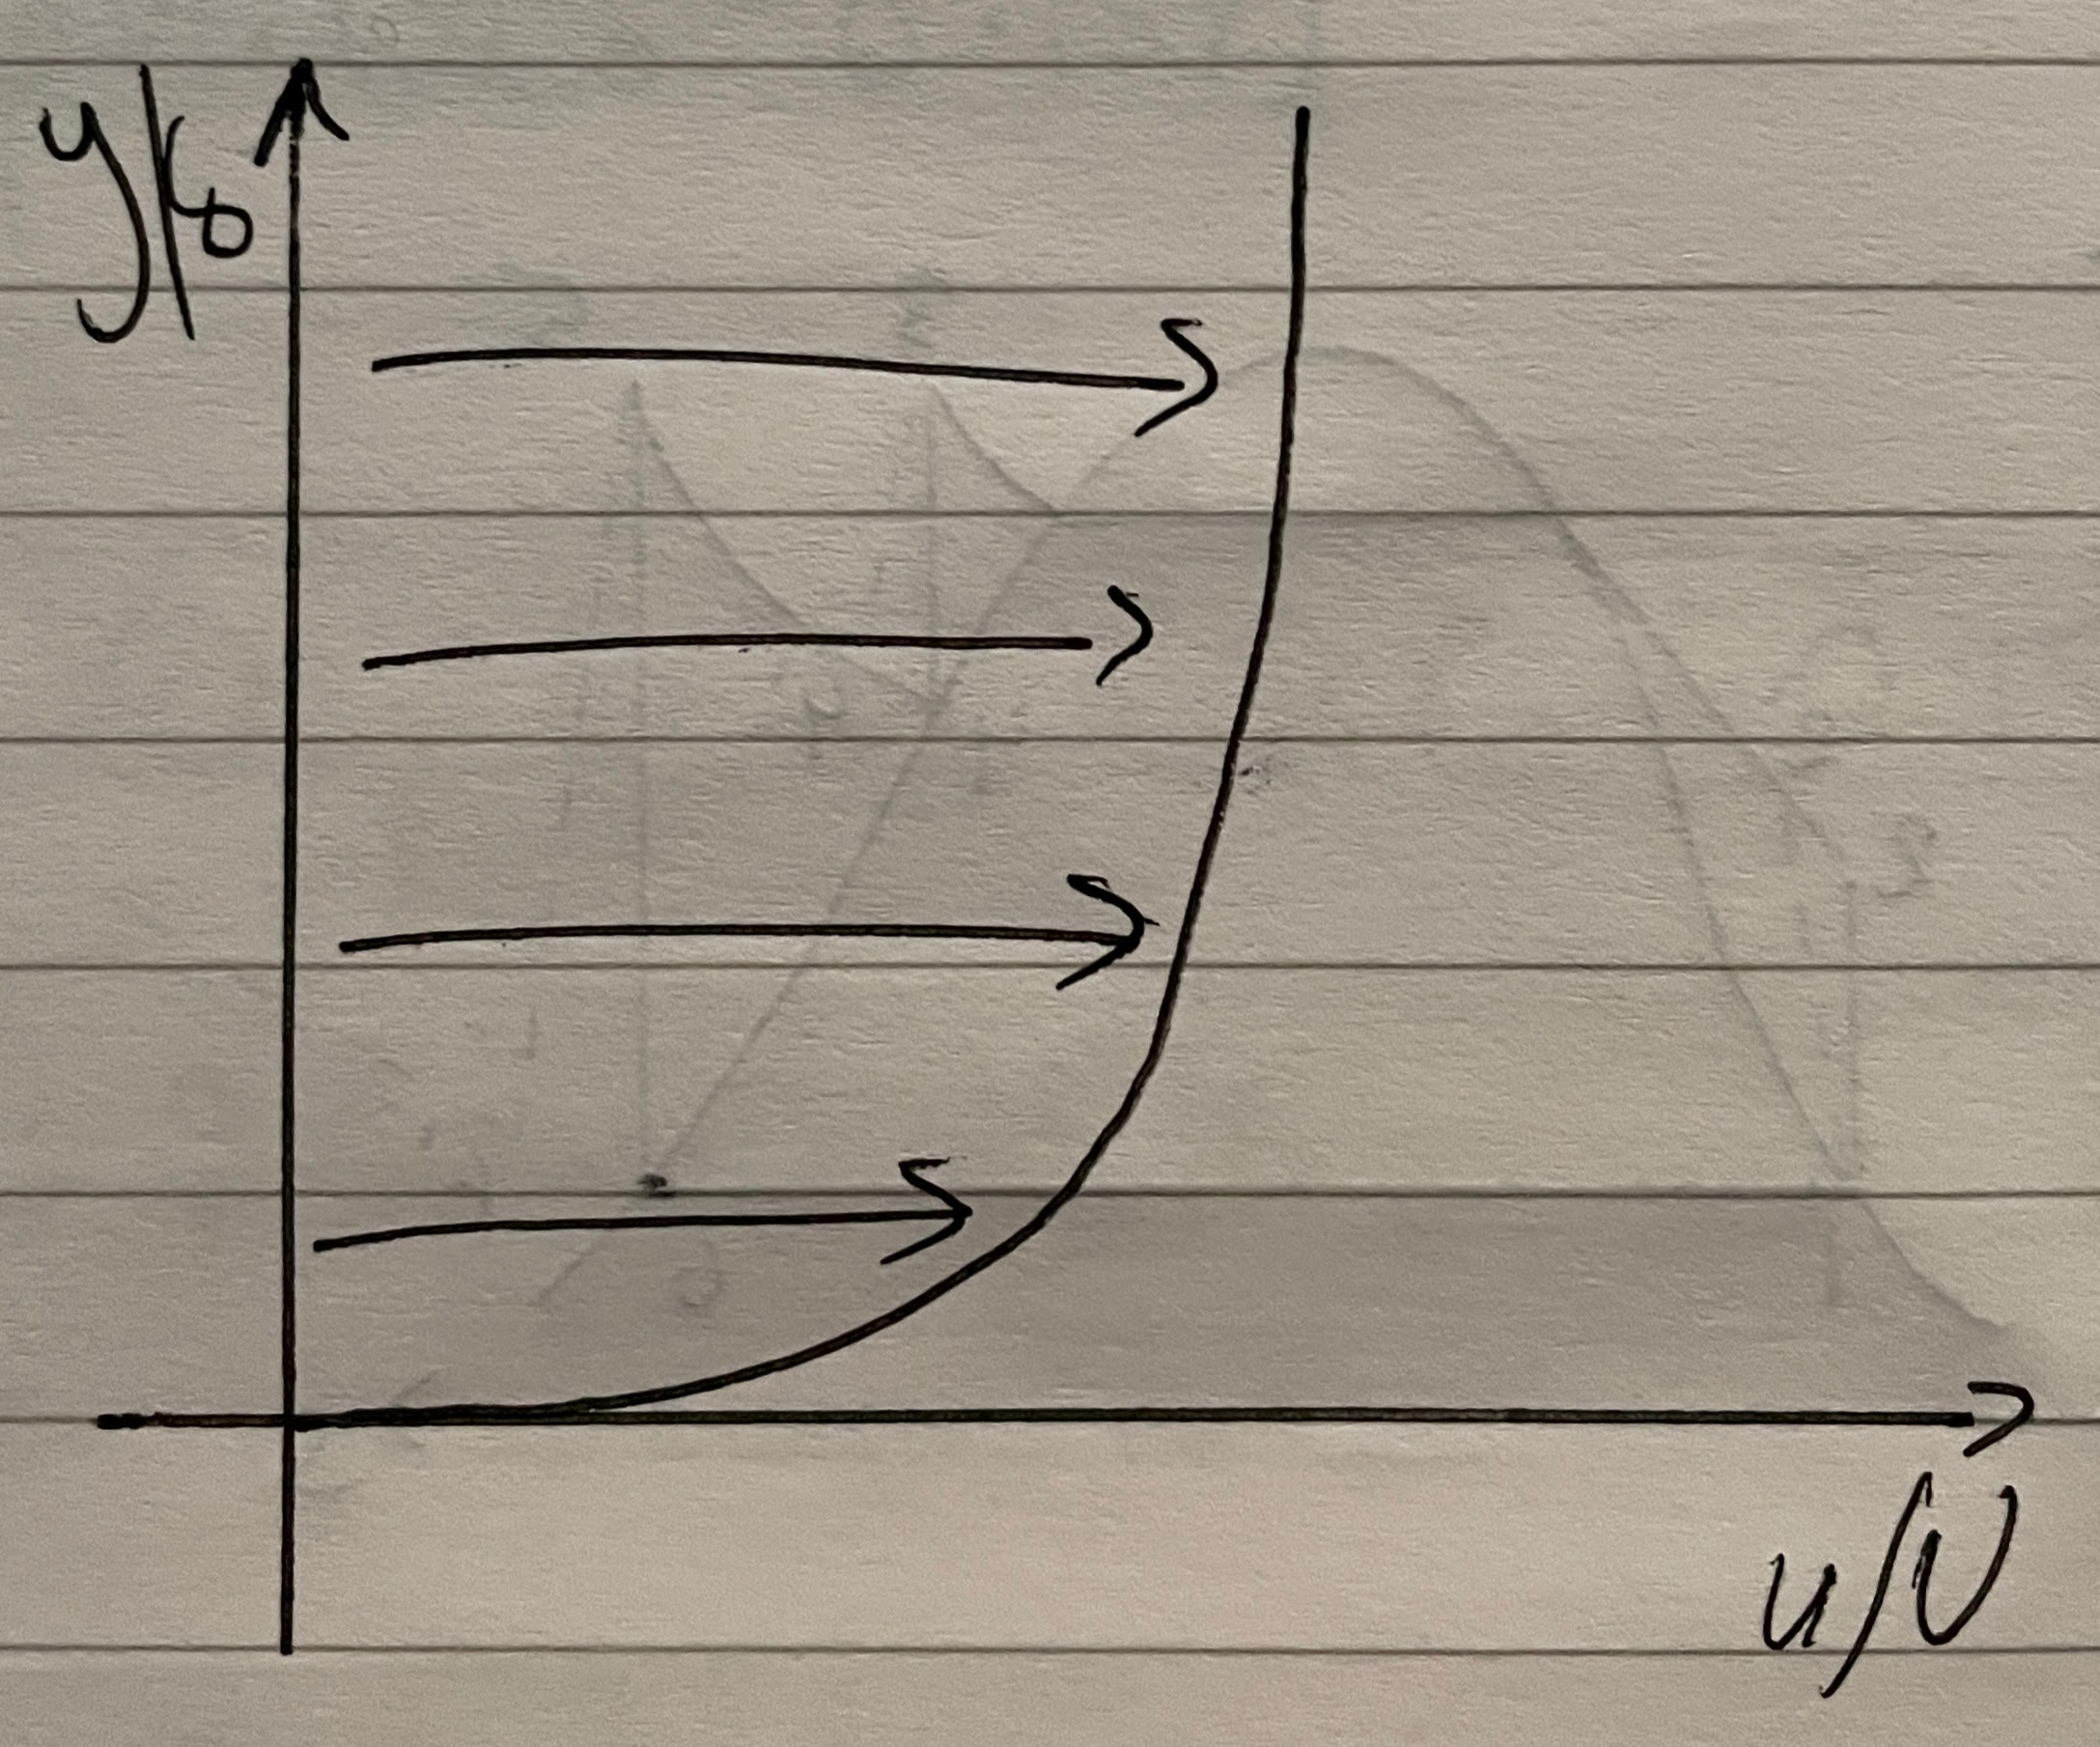
\includegraphics[height = 5cm]{./img/q3b1.jpg}
    \caption{Graph to show boundary layer velocity profile upstream.}
    \label{fig:q3b1}
\end{figure}
\begin{figure}[H]
    \centering
    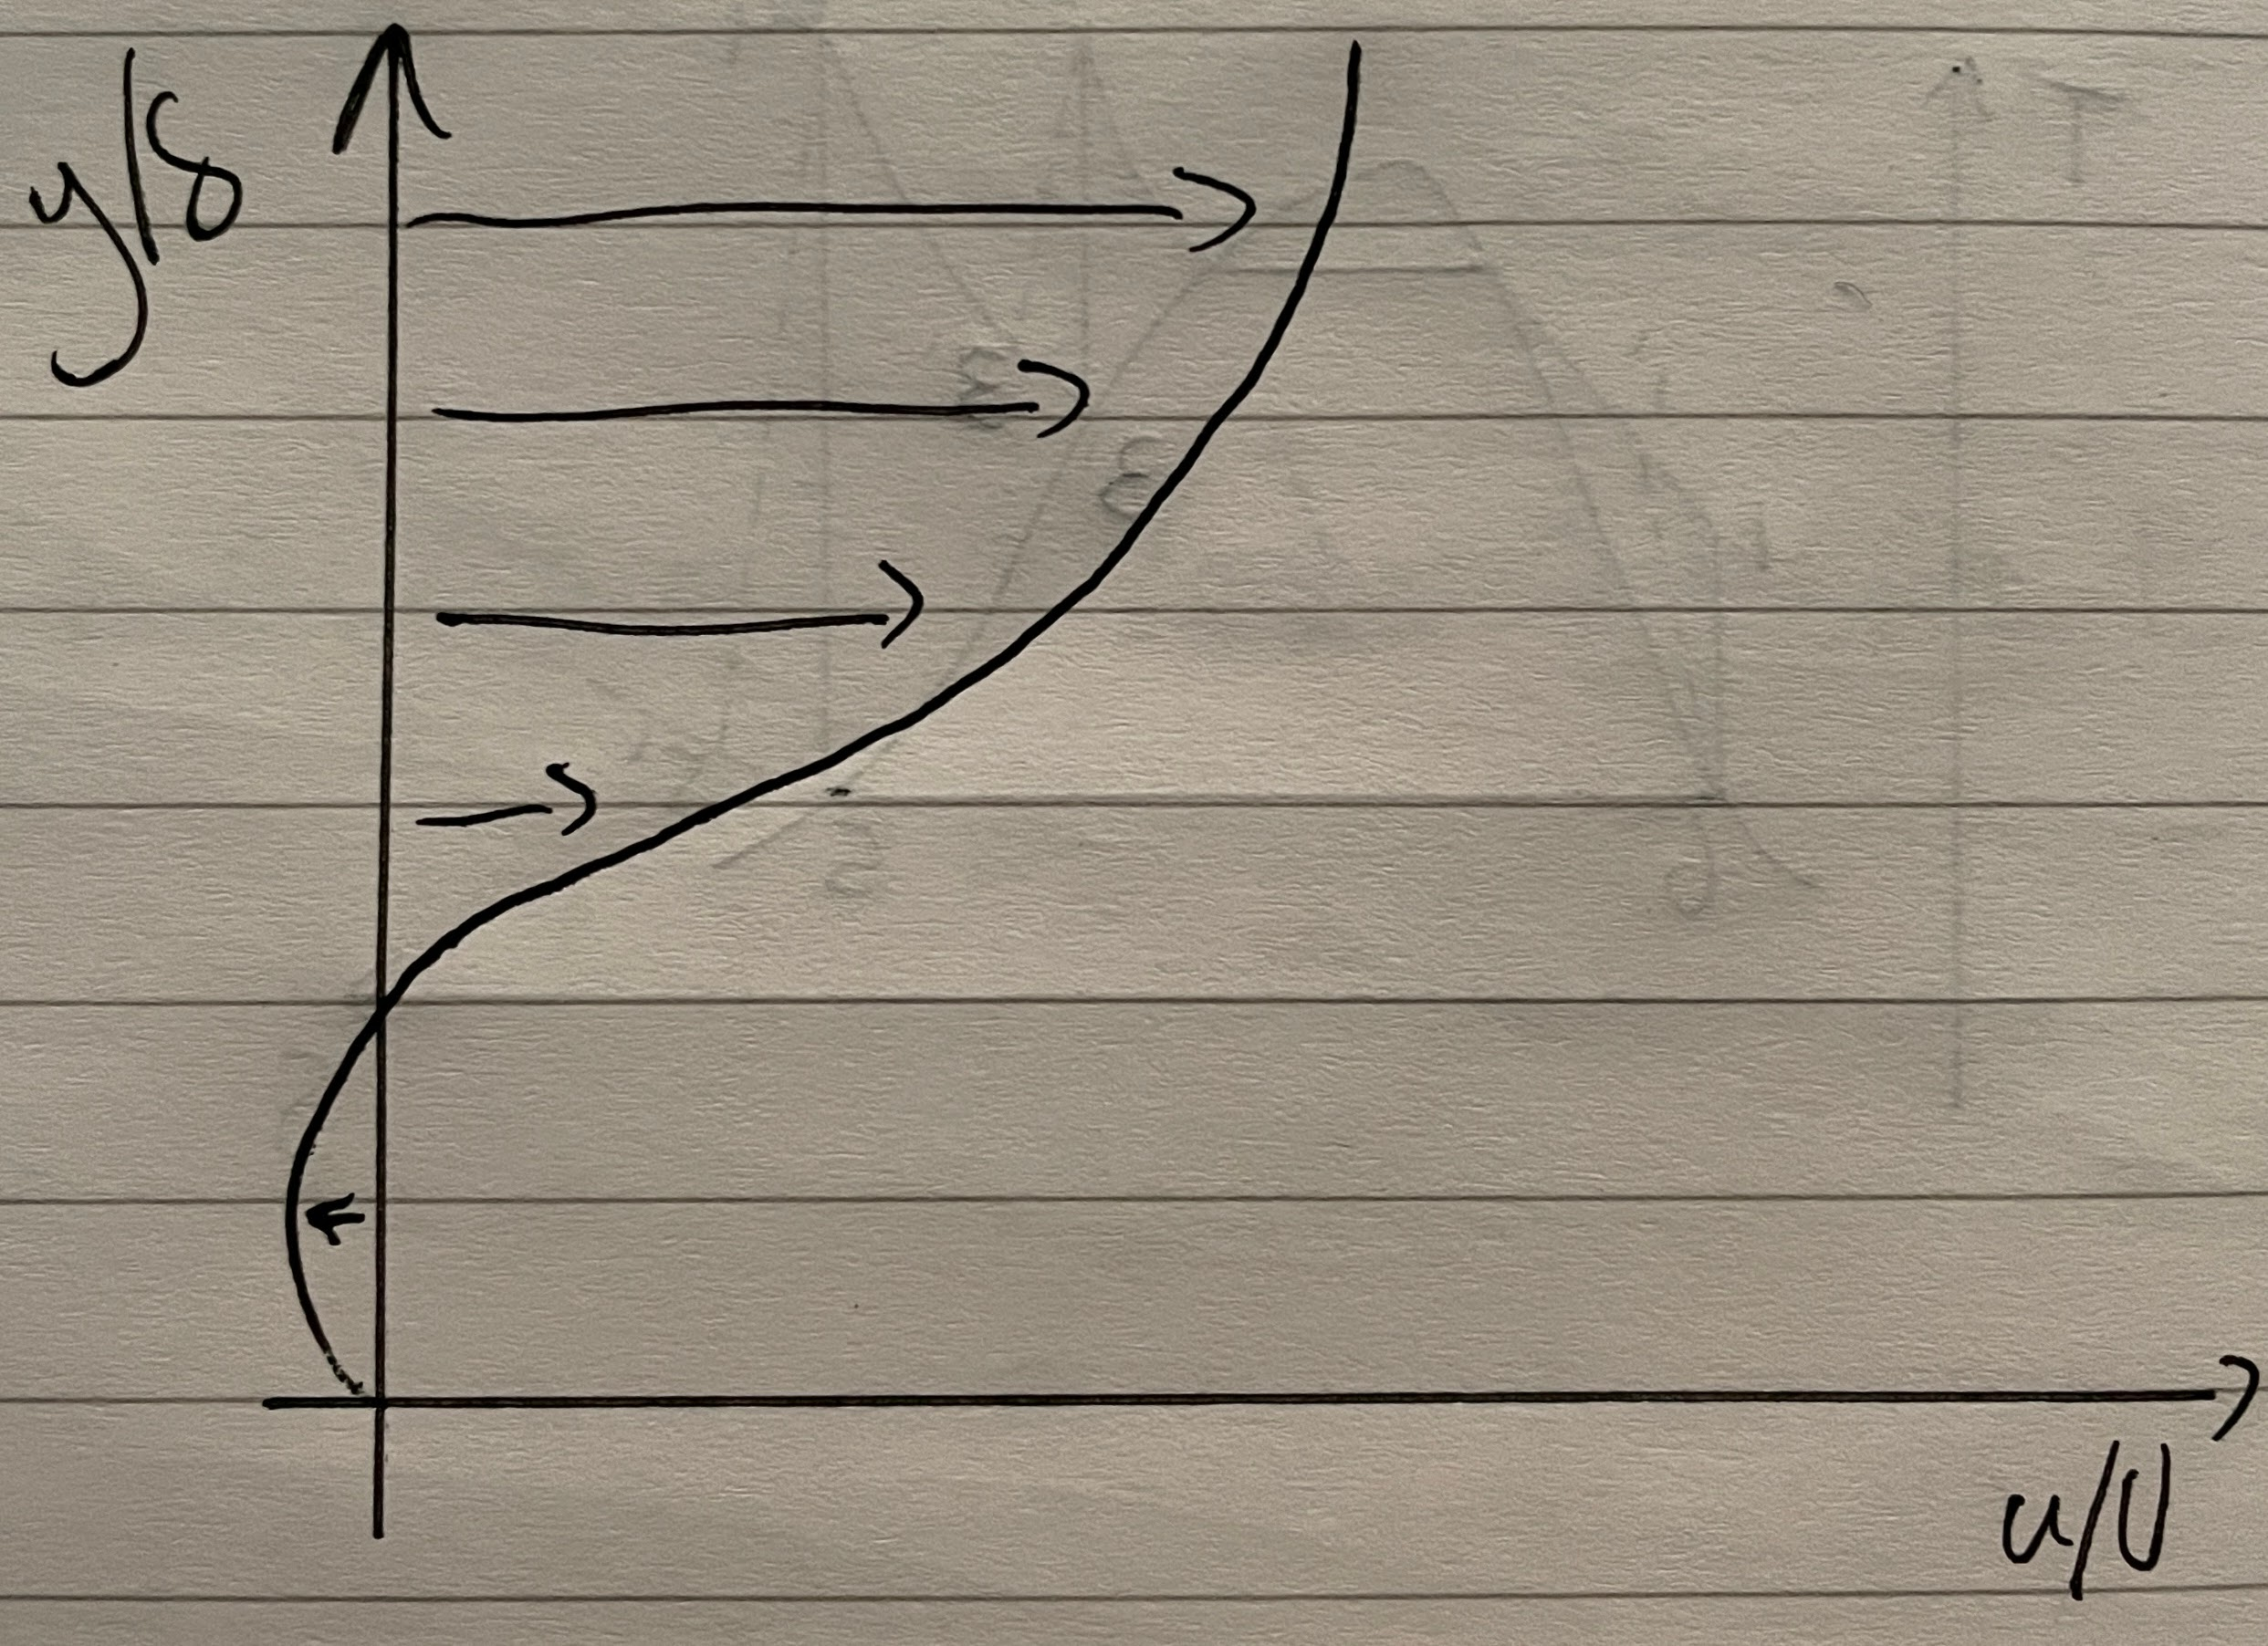
\includegraphics[height = 5cm]{./img/q3b2.jpg}
    \caption{Graph to show boundary layer velocity profile downstream.}
    \label{fig:q3b2}
\end{figure}
\section{Question 4}
\subsection{a}
The balanced reaction equation takes the general form:
\begin{align}
    \ce{C_x H_y} + a \left(\ce{O2} + \ce{3.76N2}\right)&\longrightarrow b \ \ce{CO2} + c \ \ce{H2O} + 3.76 d \ \ce{N2} + e \ \ce{O2}\\
\end{align}
Since this is the reaction of methane with 110\% stoichiometric air, we can put in our values and balance our equation
\begin{equation}
    \ce{CH4} + 2.2\left(\ce{O2} + \ce{3.76N2}\right)\longrightarrow \ce{CO2} + \ce{2H2O} + \ce{8.272N2} + \ce{0.2O2}
\end{equation}
\subsection{b}
The air-fuel ratio on a mass basis can be found using \ref{eq:q4b1}
\begin{align}
    AF &= \bar{AF} \times \dfrac{M_{air}}{M_{fuel}} \label{eq:q4b1}
\end{align}
Where and $\bar{AF}$ is volumetric air ratio and $M$ is the molar mass. Assuming that the air only consists of oxygen and nitrogen, we can input molar masses from the property tables into the \ref{eq:q4b1}:
\begin{align}
    AF &= \dfrac{2.2\left(1 + 3.76\right)}{1} \times  \dfrac{\left(\dfrac{32+3.76\left(28.01\right)}{4.76}\right)}{16.04}\\
    AF &= \SI{18.8}{\kg\of{air}\per\kg\of{fuel}}
\end{align}
\subsection{c}
\begin{figure}[H]
    \centering
    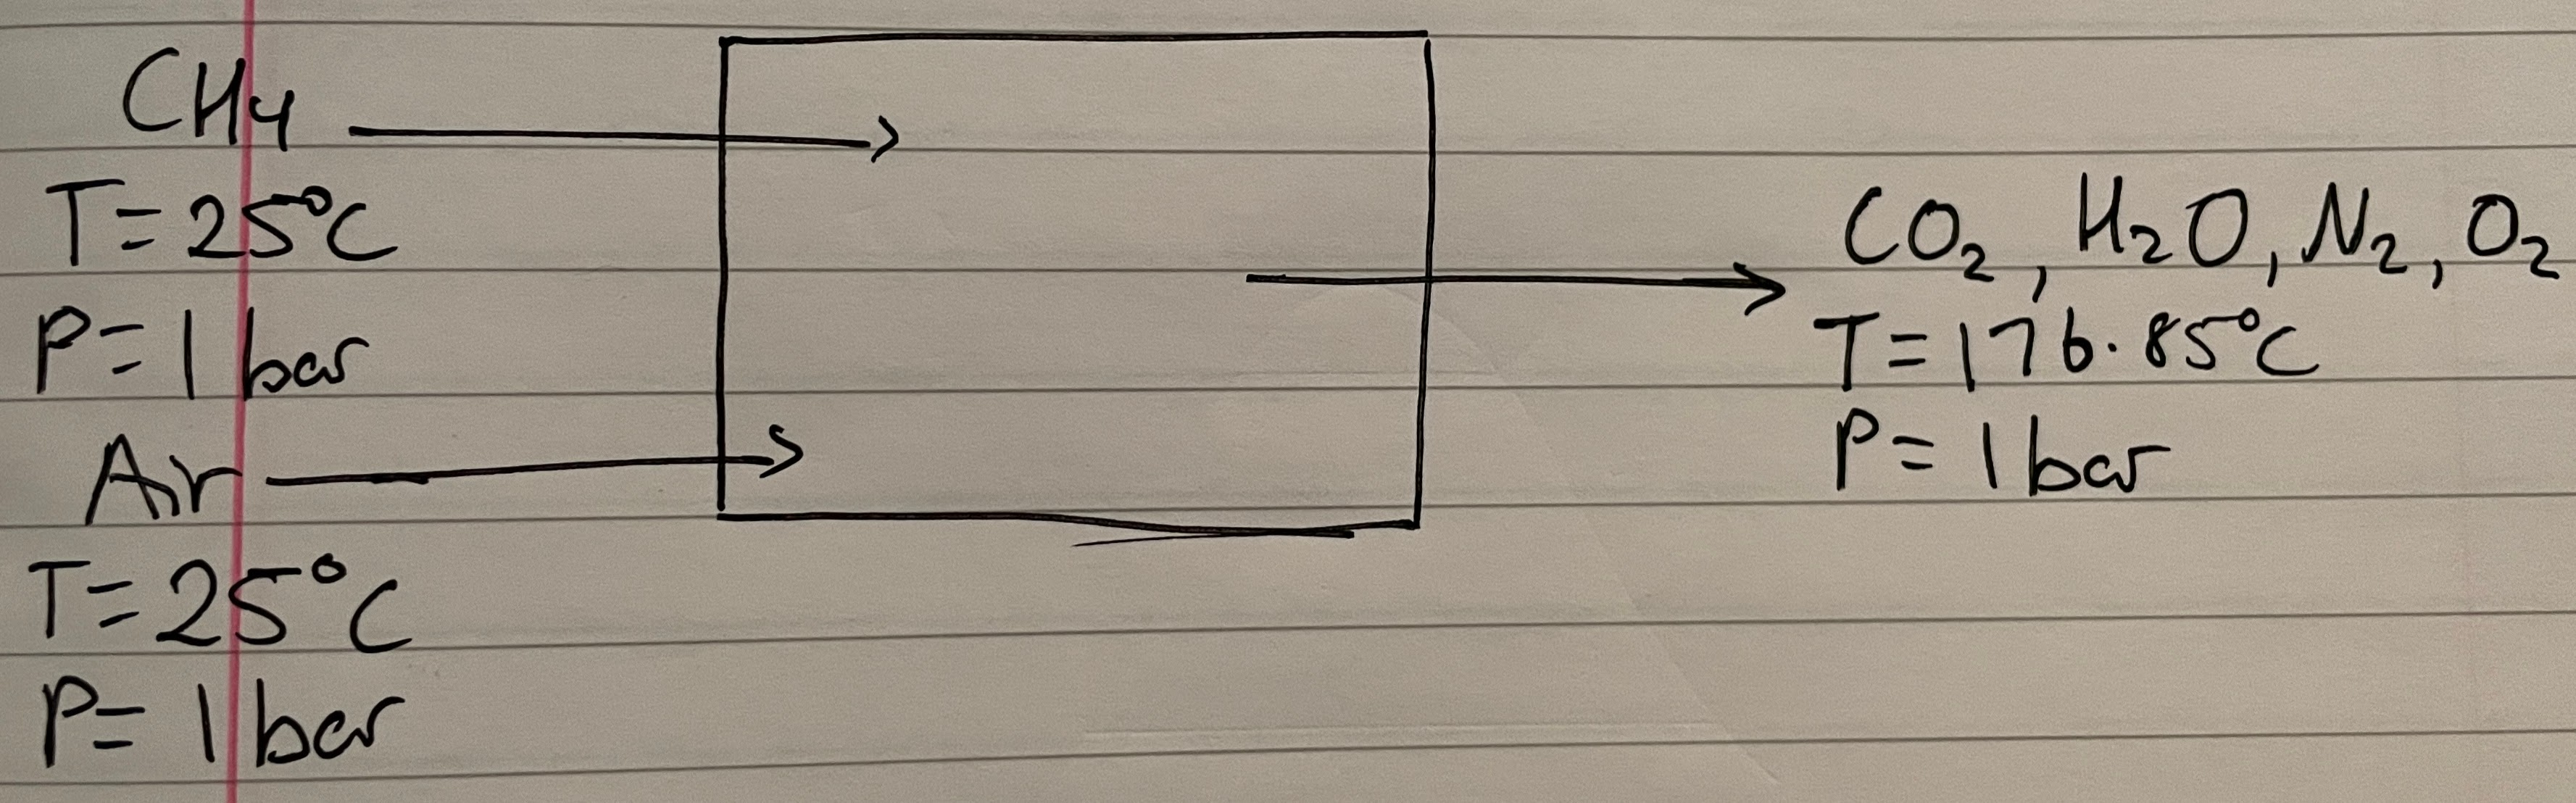
\includegraphics[height = 4cm]{./img/q4c.jpg}
    \caption{Diagram to show combustion.}
    \label{fig:q4c}
\end{figure}
Temperature of reactants is given as \SI{298}{\kelvin}. Temperature of products was selected to be \SI{450}{\kelvin} (\SI{176.85} {\celsius}). Assumptions:
\begin{itemize}
    \item Control volume is in a steady state
    \item \ce{N2} is an inert gas
    \item Isobaric process
    \item Neglect kinetic and potential energies of the particles
    \item No mechanical work
\end{itemize}
We also know that there is 3.76 moles of nitrogen for every mole of oxygen in the air. Standard enthalpy of reaction is given as:
\begin{equation}
    \Delta \bar{h}_r = \sum_{\textrm{products}} n_i \bar{h}_{i}(T) - \sum_{\textrm{reactants}} n_i \bar{h}_{i}(T)
\end{equation}
Reaction equation:
\begin{equation}
    \ce{CH4} + 2.2\left(\ce{O2} + \ce{3.76N2}\right)\longrightarrow \ce{CO2} + \ce{2H2O} + \ce{8.272N2} + \ce{0.2O2}
\end{equation}
Calculating the sum of the products using the formula $\bar{h} = \bar{h}^o_{f,i} + \Delta \bar{h}_i(T)$:
\begin{multline}
    \sum_{\textrm{reactants}} n_i \bar{h}_{i}(T) = \left[ \bar{h}^o_f + \bar{h}(450) - \bar{h}(289)\right]_{\ce{CO2}} + 2 \left[ \bar{h}^o_f + \bar{h}(450) - \bar{h}(289)\right]_{\ce{H2O}} \\ + 8.272 \left[\bar{h}(450) - \bar{h}(289)\right]_{\ce{N2}} + 0.2 \left[ \bar{h}(450) - \bar{h}(289)\right]_{\ce{O2}}
\end{multline}
Using table values:
\begin{multline}
    \sum_{\textrm{reactants}} n_i \bar{h}_{i}(T) = \left[-393520 + 15483 - 9369\right] + 2 \left[ -241820 + 15080 - 9904\right] \\ + 8.272 \left[13105 -8669\right] + 0.2 \left[13228-8682\right]
\end{multline}
Calculating the sum of the reactants using standard enthalpies of reaction:
\begin{equation}
    \sum_{\textrm{products}} n_i \bar{h}_{i}(T) = \left[\bar{h}^o_{f}\right]_{\ce{CH4}} + 2.2\left[\bar{h}^o_{f}\right]_{\ce{O2}} + 8.272\left[\bar{h}^o_{f}\right]_{\ce{N2}}
\end{equation}
Using table values:
\begin{equation}
    \sum_{\textrm{products}} n_i \bar{h}_{i}(T) = \left[-74870\right] + 2.2\left[ 0 \right] + 8.272\left[0\right]
\end{equation}
Hence, the final enthalpy of reaction is:
\begin{equation}
    \Delta \bar{h}_r = -823090.208 - \left( - 74870\right) = \SI{-748220.208}{\kilo\joule\per\kilo\mol }
\end{equation}
\subsection{d}
We know that all the water obtained in the combustion is a vapour, hence we can deduce that the enthalpy of reaction value obtained is the lower heating value.
\section{Question 5}
\subsection{a}
\begin{figure}[H]
    \centering
    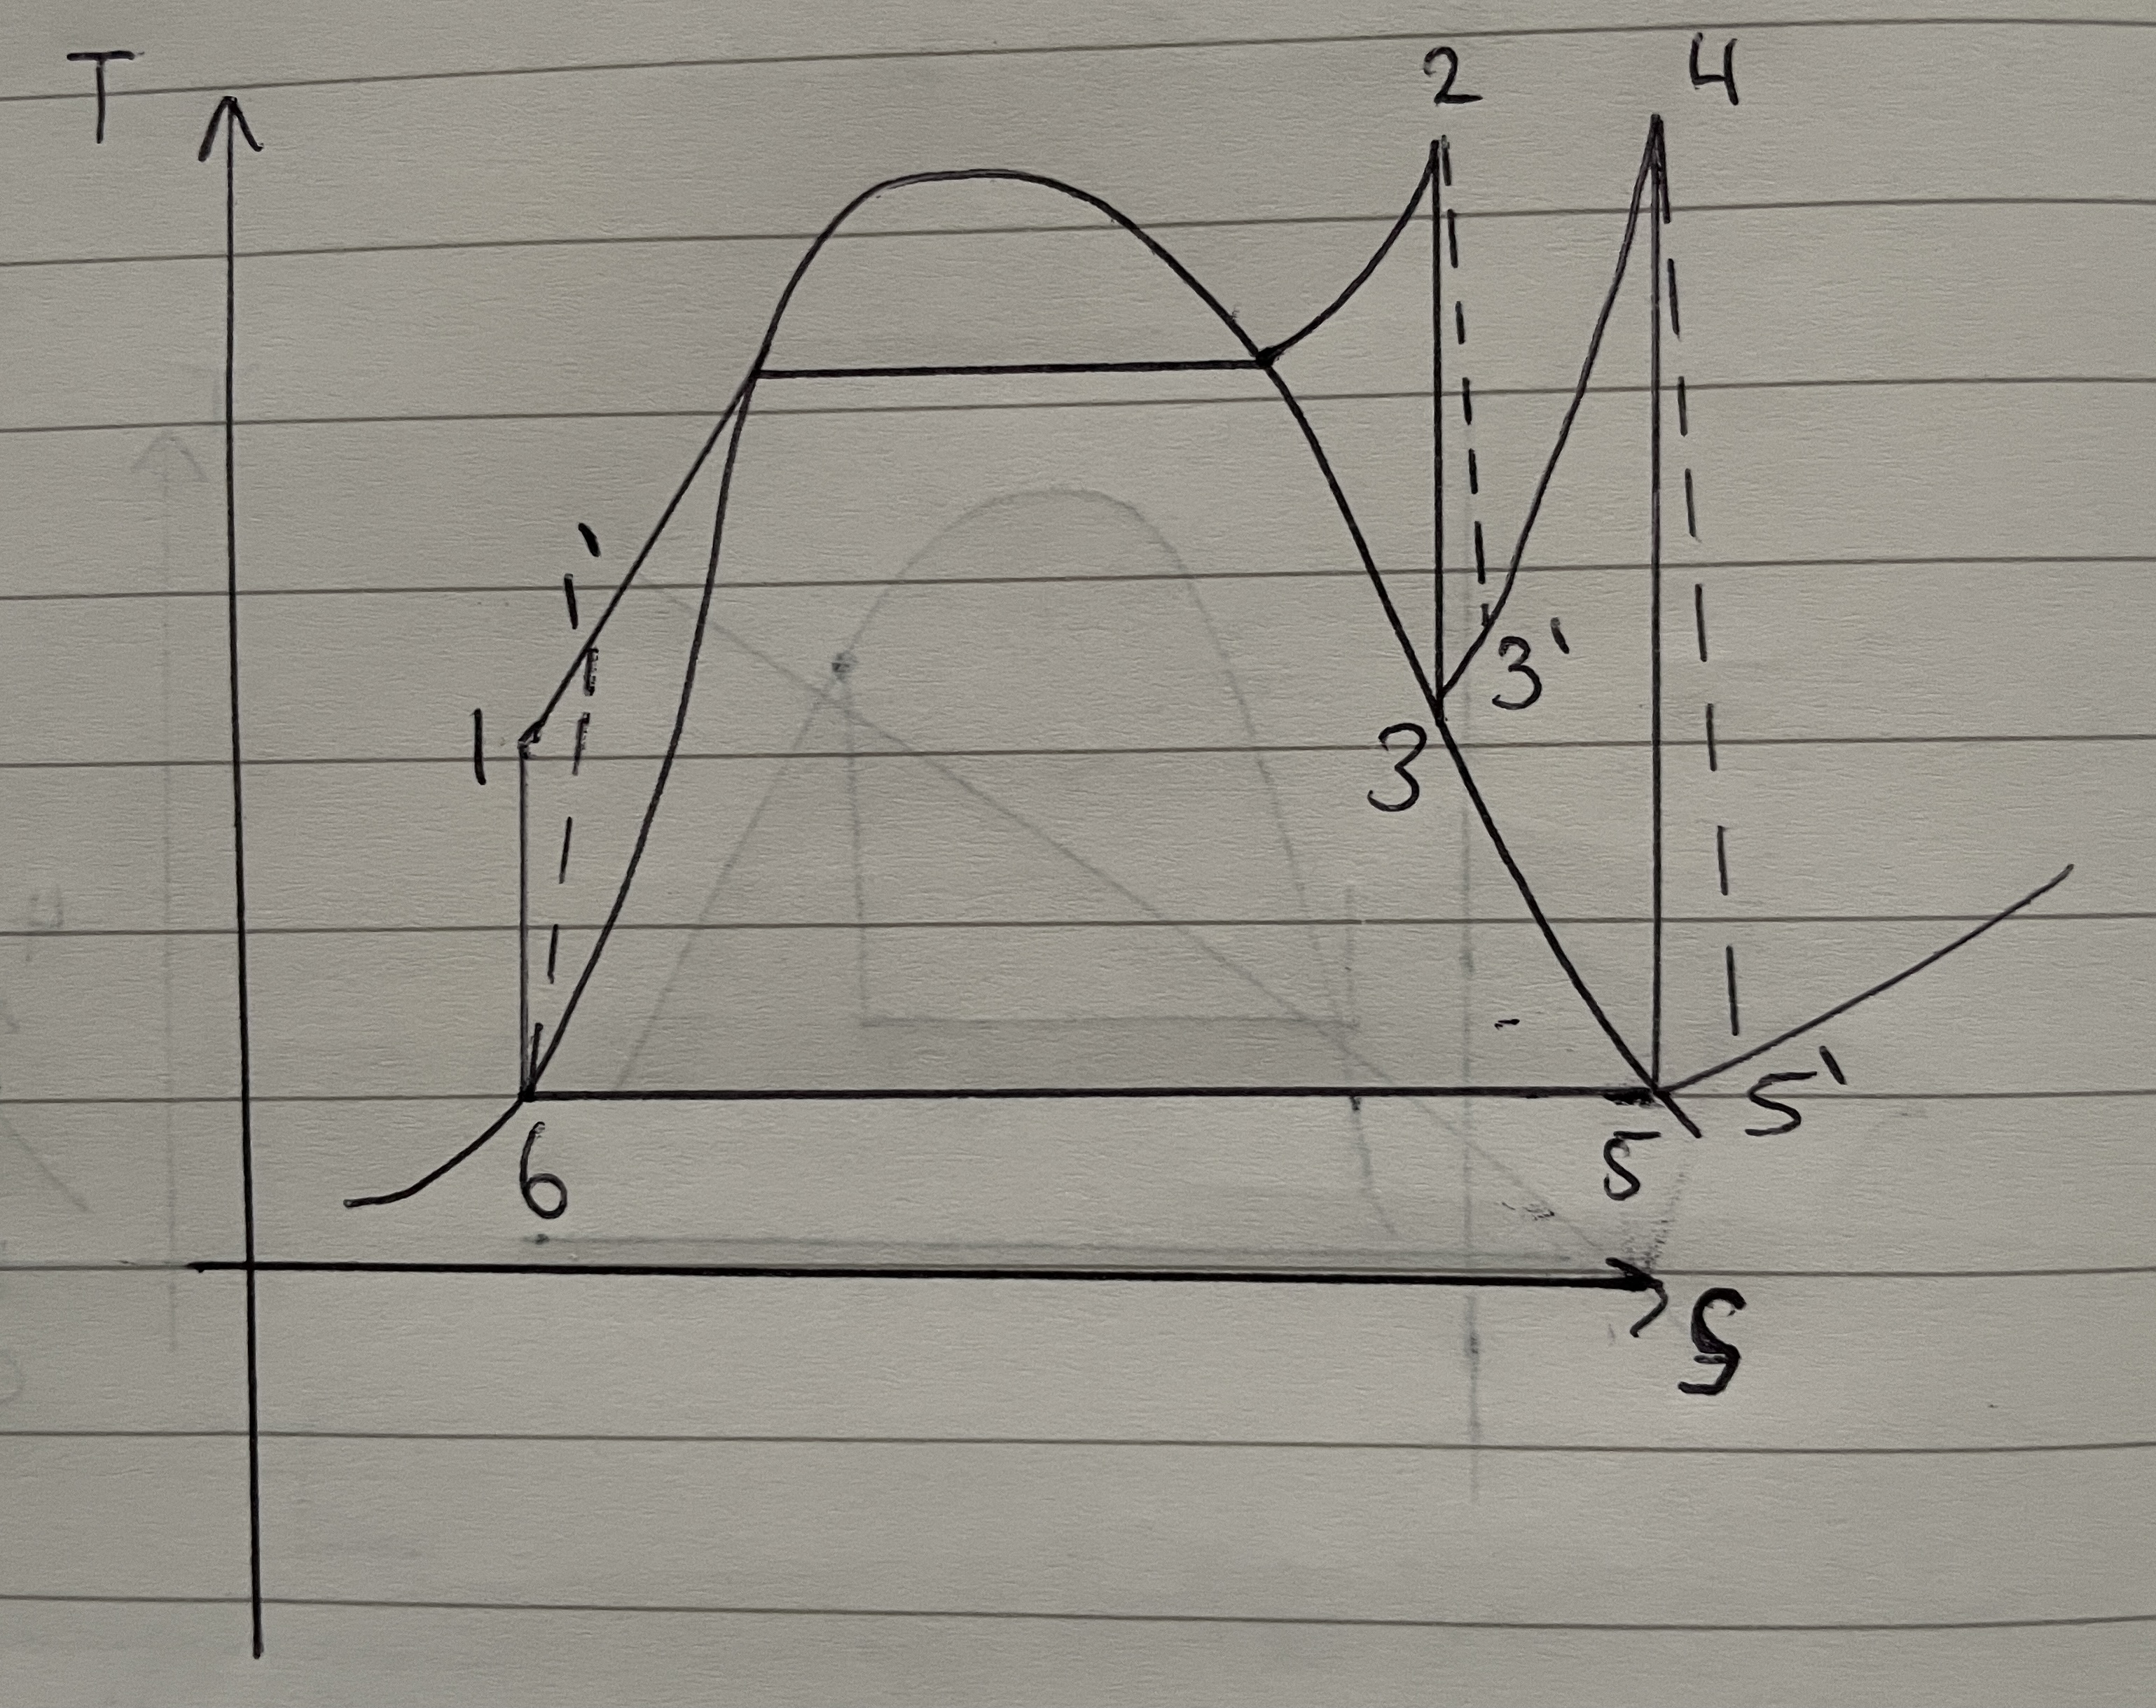
\includegraphics[height = 8cm]{./img/q5a.jpg}
    \caption{Graph to show Rankine cycle on T-s diagram.}
    \label{fig:q5a}
\end{figure}
In an ideal Rankine reheat cycle, we would see that the expansion and compression processes are reversible and isentropic. These are shown as straight vertical lines from 6 - 1 (pump compression), 2 - 3 and 4 - 5 (turbine expansion). However, in an actual Rankine reheat cycle, we will have irreversible losses present. For a pump, work must be done to overcome frictional forces. For a turbine, heat transfer from the turbine to the surroundings represents a loss. This process of transfer of energy as work results in entropy being produced within the system, hence we would see the entropy increase for these processes. These have been represented as the curved lines 6 - 1', 2 - 3' and 4 - 5'. 
\subsection{b}
All components in the Rankine reheat cycle are steady flow devices. Neglect kinetic and potential energy changes as they are usually small relative to the work and heat transfer terms. Starting with SFEE formula:
\begin{align}
    \dot{Q}_{in} + \dot{W}_{in} + \dot{m}_1 h_1 = \dot{Q}_{out} + \dot{W}_{out} + \dot{m}_2 h_2
\end{align}
$\dot{m}_1 = \dot{m}_2 = \dot{m}$. Dividing by $\dot{m}$:
\begin{align}
    q_{in} + w_{in} + h_1 = q_{out} + w_{out} + h_2
\end{align}
The thermal efficiency is given by:
\begin{equation}
    \eta_{th} = \dfrac{w_{net}}{q_{in}} = \dfrac{w_{turbines} - w_{pump}}{q_{in}}
\end{equation}
We know that the total heat input will come from the primary heating stage and the reheating stage, hence:
\begin{align}
    q_{in} = q_{\textrm{primary}} + q_{\textrm{reheat}} = \left(h_2 - h_1\right) + \left(h_4 - h_3\right)
\end{align}
Total power output from the turbines can be calculated as:
\begin{align}
    w_{turbines} = w_{turb1} + w_{turb2} = \left(h_2 - h_3\right) + \left(h_4 - h_5\right)
\end{align}
Pump power can be calculated as:
\begin{align}
    w_{pump} = \left(h_1 - h_6\right)
\end{align}
Therefore, the thermal efficiency is:
\begin{align}
    \eta_{th} = \dfrac{w_{net}}{q_{in}} = \dfrac{\left(h_2 - h_3\right) + \left(h_4 - h_5\right) - \left(h_1 - h_6\right)}{\left(h_2 - h_1\right) + \left(h_4 - h_3\right)}
\end{align}
Let us look at the principal states at each stage on our T-s diagram. State 2 (enthalpy and entropy derived from table values):
\begin{align}
    P_2 &= \SI{70}{\bar}\\
    T_2 &= \SI{500}{\celsius}\\
    h_2 &= \SI{3410}{\kilo\joule\per\kg}\\
    s_2 &= \SI{6.796}{\kilo\joule\per\kg\per\kelvin}
\end{align}
At state 3, our entropy is the same as that at state 2, hence using table values:
\begin{align}
    P_3 &= \SI{5}{\bar}\\
    s_3 &= \SI{6.796}{\kilo\joule\per\kg\per\kelvin}
\end{align}
Finding the quality:
\begin{align}
    6.796 &= 1.860 + 4.962x\\
    x &= 0.99476
\end{align}
Therefore:
\begin{align}
    h_3 &= 640 + 2109\left(0.99476\right)\\
    h_3 &= \SI{2737.95}{\kilo\joule\per\kg}
\end{align}
State 4 (table values):
\begin{align}
    P_4 &= \SI{5}{\bar}\\
    T_4 &= \SI{500}{\celsius}\\
    h_4 &= \SI{3484}{\kilo\joule\per\kg}\\
    s_4 &= \SI{8.087}{\kilo\joule\per\kg\per\kelvin}
\end{align}
At state 5, our entropy is the same as that at state 4, hence using table values:
\begin{align}
    P_5 &= \SI{0.08}{\bar}\\
    s_5 &= \SI{8.087}{\kilo\joule\per\kg\per\kelvin}
\end{align}
Finding the quality:
\begin{align}
    8.087 &= 0.593 + 7.634x\\
    x &= 0.98166
\end{align}
Therefore:
\begin{align}
    h_5 &= 174 + 2404(0.98166)\\
    h_5 &= \SI{2531.949699}{\kilo\joule\per\kg}
\end{align}
State 6:
\begin{align}
    P_6 &= \SI{0.08}{\bar}\\
    s_6 &= \SI{0.593}{\kilo\joule\per\kg\per\kelvin}\\
    h_6 &= \SI{174}{\kilo\joule\per\kg}
\end{align}
State 1:
\begin{align}
    P_1 &= \SI{70}{\bar}\\
    h_1 & \approx h_6 + v_6 \left(P_1 - P_6\right)\\
    h_1 & \approx 174 + \left(1.0084\times 10^{-3}\right)\left(70-0.08\right)\left(\frac{10^5}{10^3}\right)\\
    h_1 &= \SI{181.0507}{\kilo\joule\per\kg}
\end{align}
Therefore, our thermal efficiency is:
\begin{align}
    \eta_{th} &= \dfrac{3410-2737.95+3484-2531.949-181.0507+174}{3410 -181.0507+3484-2737.95}\\
    \eta_{th} &= 0.4068 = 40.68\%
\end{align}
\subsection{c}
If the HPT and LPT do not expand isentropically, our thermal efficiency will become:
\begin{align}
    \eta_{th} = \dfrac{w_{net}}{q_{in}} = \dfrac{\left(h_2 - h_{3'}\right) + \left(h_4 - h_{5'}\right) - \left(h_{1'} - h_6\right)}{\left(h_2 - h_{1'}\right) + \left(h_4 - h_{3'}\right)}
\end{align}
As the enthalpies at the actual points is more than those at the ideal points, we see a net decrease in the thermal efficiency.
\subsection{d}
Population of my local area, Redbridge, is given as 300 thousand \cite{b2}. Therefore, the total power that needs to be generated is \SI{300}{\mega\watt}.
We know that 80\% of combustion heat is used to generate vapour for the steam turbine, hence:
\begin{align}
    0.8 \times 748220.208 = \SI{598576.1664}{\kilo\joule\per\kilo\mol }
\end{align}
Next, to find the mass flow rate of the steam, we can use the following formula:
\begin{align}
    \dot{W}_{net} &= \dot{W}_{turbines} - \dot{W}_{pump}\\
    \dot{W}_{net} &= \dot{m} \left(h_2 - h_3\right) + \left(h_4 - h_5\right) - \left(h_1 - h_6\right)\\
    \dot{m} &= \dfrac{\dot{W}_{net}}{\left(h_2 - h_3 + h_4 - h_5 - h_1 + h_6\right)}\\
    \dot{m} &= \dfrac{3\times 10^5}{3410-2737.95+3484-2531.949-181.0507+174}\\
    \dot{m} &= \SI{185.523}{\kg\per\s} \label{eq:q5d1}
\end{align}
The energy into our boiler from initial and reheat stages is:
\begin{align}
    \dfrac{\dot{Q}_{in}}{\dot{m}} &= \left(h_2 - h_1\right) + \left(h_4 - h_3\right)\\
    \dot{Q}_{in} &= \left(185.523\right)\left(3410 -181.0507+3484-2737.95\right)\\
    \dot{Q}_{in} &= \SI{737453.7391}{\kilo\joule\per\second}
\end{align}
Now we can calculate the mass flow rate of fuel required to supply the boiler with the above required rate of energy.
\begin{align}
    \dot{m}_{\ce{CH4}} &= \dfrac{\dot{Q}_{in}}{Q_{vapour}}\\
    \dot{m}_{\ce{CH4}} &= \dfrac{737453.7391}{598576.1664}\\
    \dot{m}_{\ce{CH4}} &= \SI{1.232}{\kilo\mol\per\second}
\end{align}
\section{Question 6}
\subsection{a}
A heat exchange efficiency of 90\% is assumed. Heat transfer out of the condenser is given by:
\begin{align}
    \dfrac{\dot{Q}_{out}}{\dot{m}} &= h_5 - h_6
\end{align}
Mass flow rate of the steam in the condenser was already calculated as \SI{185.523}{\kg\per\s} in \ref{eq:q5d1} and since our efficiency is only 90\%, $\dot{Q}_{out} =0.9\times \dot{Q}$. Therefore:
\begin{align}
    \dfrac{0.9\times\dot{Q}}{185.523} &= 2531.95 - 174\\
    \dot{Q} &= \SI{486059.9532}{\kilo\joule\per\second}
\end{align}
Let us now look at the water entering the condenser:
\begin{align}
    \dfrac{\dot{Q}}{\dot{m}_{cw}} &= h_7 - h_9\\
    \dot{m}_{cw} &= \dfrac{\dot{Q}}{h_7 - h_9}
\end{align}
State 7 (from tables):
\begin{align}
    T_7 &= \SI{40}{\celsius}\\
    h_7 &= \SI{167.5}{\kilo\joule\per\second}
\end{align}
State 9:
\begin{align}
    T_9 &= \SI{25}{\celsius}\\
    h_9 &= \SI{104.8}{\kilo\joule\per\second}
\end{align}
Therefore:
\begin{align}
    \dot{m}_{cw} &= \dfrac{\dot{Q}}{h_7 - h_9}\\
    \dot{m}_{cw} &= \dfrac{486059.9532}{167.5 - 104.8}\\
    \dot{m}_{cw} &= \SI{7752.152}{\kg\per\second} \label{eq:q6b1}
\end{align}
\subsection{b}
Mass flow rate of air can be calculated using the following assumptions:
\begin{itemize}
    \item Neglect kinetic and potential energies
    \item Isobaric process
    \item The control volume is in a steady state
\end{itemize}
Mass balance of dry air in the cooling tower:
\begin{align}
    \dot{m}_{10a} = \dot{m}_{11a} = \dot{m}_{a}
\end{align}
Mass balance of water in the condenser:
\begin{align}
    \dot{m}_7 &= \dot{m}_8 + \dot{m}_9\\
    \dot{m}_8 &= \dot{m}_7 - \dot{m}_9
\end{align}
Mass balance of the cooling tower:
\begin{align}
    \dot{m}_7 + \dot{m}_8 + \dot{m}_{10} &= \dot{m}_9 + \dot{m}_{11}\\
    \dot{m}_7 - \dot{m}_9 + \dot{m}_8 &= \dot{m}_11 - \dot{m}_{10}\\
    2\dot{m}_8 &= \dot{m}_{11} - \dot{m}_{10}\\
    \therefore \dot{m}_8 &= \dfrac{\dot{m}_a\left(\omega_{11} - \omega_{10}\right)}{2}
\end{align}
We also know that:
\begin{align}
    \dot{m}_{10} = \dot{m}_a \left(1 + \omega_{10}\right) \label{eq:q6b2}
\end{align}
Let us now look at the steady state energy equation:
\begin{align}
    0 &= \dot{Q}_{net} - \dot{W}_{net} + \dot{m}_7 h_7 + \dot{m}_8 h_8 -\dot{m}_9 h_9 + \left[\dot{m}_{10a} h_{10a} + \dot{m}_{10} h_{10}\right] - \left[\dot{m}_{11a} h_{11a} + \dot{m}_{11} h_{11}\right]\\
    0 &= \dot{m}_{cw} \left(h_7 - h_9\right) + \dfrac{h_8 \dot{m}_a\left(\omega_{11} - \omega_{10}\right)}{2} + \dot{m}_a \left[h_{10a} + \omega_{10}h_{10}\right] - \dot{m}_a \left[h_{11a} + \omega_{11}h_{11}\right]\\
    0 &=\dot{m}_{cw} \left(h_7 - h_9\right) + \dot{m}_a \left[\dfrac{h_8 \left(\omega_{11}- \omega_{10}\right)}{2} + h_{10a} + \omega_{10}h_{10}- h_{11a} - \omega_{11}h_{11} \right]\\
    \dot{m}_a &= \dfrac{\dot{m}_{cw} \left(h_9 - h_7\right)}{\dfrac{h_8 \left(\omega_{11}- \omega_{10}\right)}{2} + h_{10a} + \omega_{10}h_{10}- h_{11a} - \omega_{11}h_{11}} \\label{eq:q6b1}
\end{align}
State 7 (fusion, values taken from tables, all pressures at 1 bar):
\begin{align}
    T_7 &= \SI{40}{\celsius}\\
    h_7 &= \SI{167.5}{\kilo\joule\per\kg}
\end{align}
State 8 and 9:
\begin{align}
    T_{8,9} &= \SI{25}{\celsius}\\
    h_{8,9} &= \SI{104.8}{\kilo\joule\per\kg}
\end{align}
State 10:
\begin{align}
    T_{10} &= \SI{25}{\celsius}\\
    h_{10} &= \SI{2547.2}{\kilo\joule\per\kg}
\end{align}
State 10 (air):
\begin{align}
    T_{10a} &= \SI{25}{\celsius}\\
    h_{10a} &= \SI{298.3326}{\kilo\joule\per\kg}\\
    p_v &= 0.3 \times p_{g,\SI{25}{\celsius}}\\
    p_v &= 0.3 \times 0.03169\\
    p_v &= \SI{0.009507}{\bar}\\
    \omega_{10} &= 0.622 \cdot \dfrac{0.009507}{1 - 0.009507}\\
    \omega_{10} &= \SI{5.9701e-3}{}
\end{align}
State 11:
\begin{align}
    T_{11} &= \SI{36}{\celsius}\\
    h_{11} &= \SI{2567.1}{\kilo\joule\per\kg}
\end{align}
State 11 (air):
\begin{align}
    T_{11a} &= \SI{36}{\celsius}\\
    h_{11a} &= \SI{309.3866}{\kilo\joule\per\kg}\\
    p_v &= 0.9 \times p_{g,\SI{36}{\celsius}}\\
    p_v &= 0.3 \times 0.05947\\
    p_v &= \SI{0.053523}{\bar}\\
    \omega_{11} &= 0.622 \cdot \dfrac{0.053523}{1 - 0.053523}\\
    \omega_{11} &= \SI{0.0352}{}
\end{align}
Substituting all values into \ref{eq:q6b1}. $\dot{m}_{cw}$ has been calculated in \ref{eq:q6b1}:
\begin{align}
    \dot{m}_a &= \dfrac{\dot{m}_{cw} \left(h_9 - h_7\right)}{\dfrac{h_8 \left(\omega_{11}- \omega_{10}\right)}{2} + h_{10a} + \omega_{10}h_{10}- h_{11a} - \omega_{11}h_{11}}\\
    \dot{m}_a &= \dfrac{7752.152\left(104.8-167.5\right)}{\dfrac{104.8\left(0.0352-\SI{5.9701e-3}{}\right)}{2} + 298.3326 + \left(\SI{5.9701e-3}{}\times 2547.2\right) - 309.3866 - \left(0.0352 \times 2567.1\right)}\\
    \dot{m}_{a} &= \SI{5729.291}{\kg\per\second}
\end{align}
Hence, mass flow rate of air from atmosphere can be calculated from \ref{eq:q6b2}:
\begin{align}
    \dot{m}_{10} &= 5729.291 \left(1 + 0.0059701\right)\\
    \dot{m}_{10} &= \SI{5762.46}{\kg\per\second}
\end{align}
\subsection{c}
A fan blowing the air out of the cooling tower would increase the exit mass flow rate. This would cause the water in the air to condense at a faster rate, leading to a reduction in the moistness of the air leaving the tower. As the flow of air is being accelerated, the air would also be cooler. This has the net effect that a larger air mass flow rate is required and the energy to be dissipated from the system would also increase as there will be a transfer from energy from the fan to the surroundings. 
\section{Question 7}
The Rankine reheat cycle is an effective energy generation method. It seeks to increase the efficiency of the Rankine cycle, which it does so successfully. Our steam is superheated to near the limit for turbines (\SI{620}{\celsius}), leading to high thermal efficiency, net work and heat input, however, this may require higher quality components and increased maintenance cycles to avoid failure. A high turbine temperature mitigates the risk of low quality at turbine exit, preventing damage to the turbine blades. Reheating the steam after the first turbine stage and passing it through a second turbine improves our cycle efficiency by around 4-5 percent. This is an effective and widely used method in steam power plants. 1-2 stages of reheat are a good compromise as more reheat cycles provide diminishing returns (more complex to reheat and costly for every reheat cycle). One more way to improve our thermal efficiency further is by using a regenerative cycle. An open feedwater heater can be added which is simple and inexpensive. Adding multiple feedwater heaters can become costly and complex, since a pump is required for each cycle. 
\begin{thebibliography}{00}
    \bibitem{b1} Pawlowicz, R. (2013) Key Physical Variables in the Ocean: Temperature, Salinity, and Density. Nature Education Knowledge 4(4):13 \url{https://www.nature.com/scitable/knowledge/library/key-physical-variables-in-the-ocean-temperature-102805293/} Accessed: 19/05/2021 00:00
    \bibitem{b2} Office of National Statistics, United Kingdom, Data Commons, \url{https://datacommons.org/tools/timeline#&place=wikidataId/Q208955&statsVar=Count_Person} Accessed 20/05/21 21:07
\end{thebibliography}
\end{document}